\chapter{Исследовательская часть}
В данном разделе будет проведено исследование процессорного времени выполнения разработанных алгоритмов.

\section{Технические характеристики}
Исследования проводились на устройстве со следующими характеристиками[3]
\begin{itemize}
\itemоперационная система: MacOS Sequoia 15.6.1 (24G90);
\itemпроцессор: Apple M3, 8 ядер;
\itemоперативная память: 16 Гигабайт, LPDDR5;
\end{itemize}	


\section{Реализация замеров}
Во время выполнения замеров устройство было подключено к источнику питанию и не выполняло сторонних процессов. Замеры проводились с помощью встроенной библиотеки \(chrono\). Для каждого размера матрицы каждого алгоритма запуск замера проводился 100 раз, после чего время выполнения усреднялось. Для проведения замеров была отключена оптимизация компилятора флагом -o0[4].
\begin{lstlisting}[language=C++, caption=Функция замера времени выполнения, captionpos=b]
 auto start = std::chrono::high_resolution_clock::now();
for (size_t j = 0; j < EXP_COUNT; j++) {
	matrix_1.multipy(matrix_2, answer);
}
auto end = std::chrono::high_resolution_clock::now();
auto duration = std::chrono::duration_cast<std::chrono::microseconds>(end-start);

\end{lstlisting}

\section{Оценка времени работы алгоритмов}
В таблице 4.1 представлены замеры процессорного времени работы алгоритмов на квадратных матрицах размером от 15 до 450 с шагом 15. Шаг выбран нечётным для того, чтобы в выборку попали как наилучшие, так и наихудшие случаи.

На рисунке 4.1 продемонстрирован график зависимости процессорного времени умножения от размера матрицы на случайных данных. В результате замеров было выяснено, что оптимизированный алгоритм Винограда работает быстрее на 15\% чем классический алгоритм Винограда, а также на 40\% чем стандартный. 

\begin{figure}[H]
	\centering
	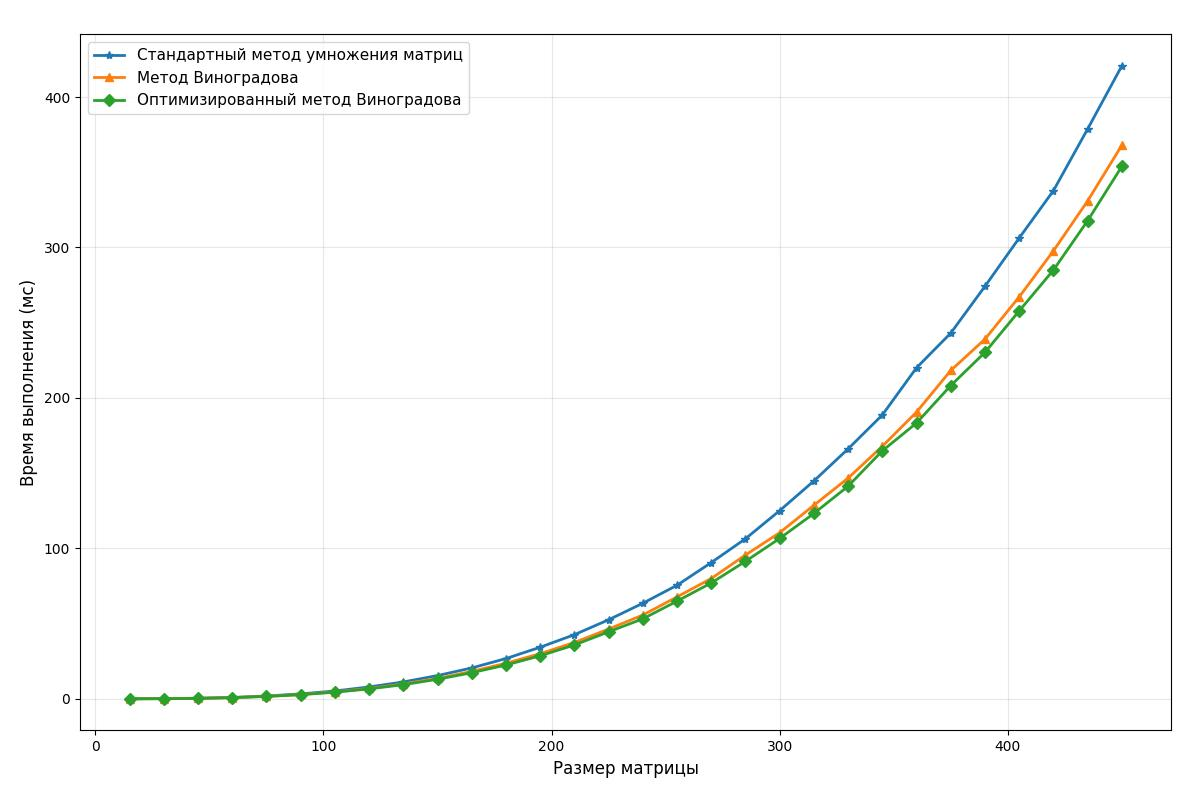
\includegraphics[width=1\textwidth]{images/AA4_1.jpg}
	\caption{Зависимость времени выполнения от размеров матриц}
	\label{fig:example_4_1}
\end{figure}


\section*{Вывод}
При реализации исследовательской части было выяснено, что оптимизированный алгоритм Винограда выполняется быстрее:
\begin{itemize}
	\itemна 5\% в худшем случае и 17\% в лучшем случае чем классический алгоритм Винограда;
	\itemна 15\% в худшем случае и 45\% в лучшем случае чем стандартный алгоритм;
\end{itemize}

\clearpage
